\begin{center}
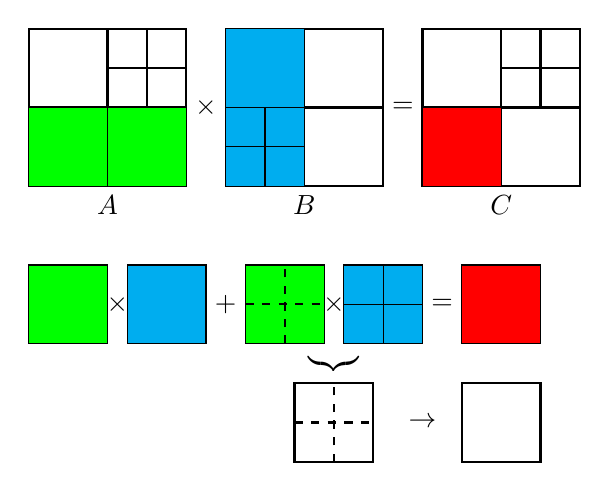
\begin{tikzpicture}[scale=0.5]
  %% matrix A
  \draw[ thick] (0,0) rectangle (4.0,4.0);
  \draw[ thick] (0,0) rectangle (2.0,2.0);
  \draw[ thick] (2.0,2.0) rectangle (4.0,4.0);
    \draw[ thick] (2.0,2.0) rectangle (3.0,3.0);
    \draw[ thick] (3.0,3.0) rectangle (4.0,4.0);
    \draw[ thick] (2.0,4.0) rectangle (3.0,3.0);
    \draw[ thick] (3.0,3.0) rectangle (4.0,2.0);
  \draw[ thick] (0,4.0) rectangle (2.0,2.0);
  \draw[ thick] (2.0,2.0) rectangle (4.0,0.0);


    \filldraw[fill=green, draw=black] (0.0,0.0) rectangle (2.0,2.0);
    \filldraw[fill=green, draw=black] (2.0,0.0) rectangle (4.0,2.0);

  %% matrix B
  \draw[ thick] (5.0,0) rectangle (9.0,4.0);
  \draw[ thick] (5.0,0) rectangle (7.0,2.0);
    \draw[ thick] (5.0,0) rectangle (6.0,1.0);
    \draw[ thick] (6.0,1.0) rectangle (7.0,2.0);
    \draw[ thick] (7.0,0) rectangle (6.0,1.0);
    \draw[ thick] (6.0,1.0) rectangle (5.0,0.0);
  \draw[ thick] (7.0,2.0) rectangle (9.0,4.0);
  \draw[ thick] (5,4.0) rectangle (7.0,2.0);
  \draw[ thick] (7.0,2.0) rectangle (9.0,0.0);

  \filldraw[fill=cyan, draw=black] (5,4.0) rectangle (7.0,2.0);
    \filldraw[fill=cyan, draw=black] (5.0,2.0) rectangle (6.0,1.0);
    \filldraw[fill=cyan, draw=black] (6.0,1.0) rectangle (7.0,2.0);
    \filldraw[fill=cyan, draw=black] (7.0,0) rectangle (6.0,1.0);
    \filldraw[fill=cyan, draw=black] (6.0,1.0) rectangle (5.0,0.0);

  %% matrix C
  \draw[thick] (10.0,0) rectangle (14.0,4.0);
  \draw[thick] (10.0,0) rectangle (12.0,2.0);
  \draw[thick] (12.0,2.0) rectangle (14.0,4.0);
    \draw[thick] (12.0,2.0) rectangle (13.0,3.0);
    \draw[thick] (13.0,3.0) rectangle (14.0,4.0);
    \draw[thick] (12.0,4.0) rectangle (13.0,3.0);
    \draw[thick] (13.0,3.0) rectangle (14.0,2.0);
  \draw[thick] (10.0,4.0) rectangle (12.0,2.0);
  \draw[thick] (12.0,2.0) rectangle (14.0,0.0);
  \filldraw[ fill=red, draw=black] (10.0,0.0) rectangle (12.0,2.0);

  %% A
  \node at (4.5,2.0) {$\times$};
  \node at (9.5,2.0) {$=$};
  \node[below] at (12.0,0.0) {$C$};
  \node[below] at (7.0,0.0) {$B$};
  \node[below] at (2.0,0.0) {$A$};

  \filldraw[fill=green, draw=black] (0.0,-4.0) rectangle (2.0,-2.0);
  \filldraw[fill=cyan, draw=black] (2.5,-4.0) rectangle (4.5,-2.0);

  \filldraw[fill=green, draw=black] (5.5,-4.0) rectangle (7.5,-2.0);
    \draw[dashed, thick] (6.5,-4.0) -- (6.5,-2.0);
    \draw[dashed, thick] (5.5,-3.0) -- (7.5,-3.0);

  \filldraw[fill=cyan, draw=black] (8.0,-4.0) rectangle (10.0,-2.0);
    \filldraw[fill=cyan, draw=black] (8.0,-4.0) rectangle (9.0,-3.0);
    \filldraw[fill=cyan, draw=black] (9.0,-3.0) rectangle (10.0,-2.0);
    \filldraw[fill=cyan, draw=black] (8.0,-2.0) rectangle (9.0,-3.0);
    \filldraw[fill=cyan, draw=black] (9.0,-3.0) rectangle (10.0,-4.0);

  \node at (2.25,-3) {$\times$};
  \node at (5.0,-3) {$+$};
  \node at (7.75,-3) {$\times$};
  \node[below] at (7.75,-4) {$\underbrace{}$};

  \node at (10.5,-3) {$=$};
  \filldraw[fill=red, draw=black] (11.0,-4.0) rectangle (13.0,-2.0);

  \draw[thick] (6.75,-7.0) rectangle (8.75,-5.0);
  \draw[dashed, thick] (7.75,-7.0) -- (7.75,-5.0);
  \draw[dashed, thick] (6.75,-6.0) -- (8.75,-6.0);

  \draw[thick] (11.0,-7.0) rectangle (13.0,-5.0);
  \node at (10.0,-6.0) {$\rightarrow$};

\end{tikzpicture}
\end{center}

